\documentclass[border=10pt]{standalone}
\usepackage{tikz}\usepackage{amsmath}
\usetikzlibrary{calc,arrows.meta}
\begin{document}
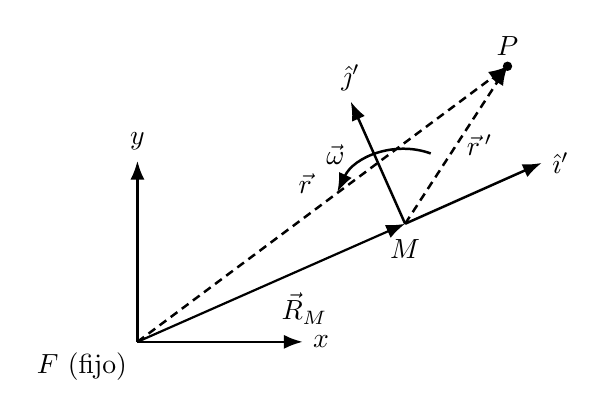
\begin{tikzpicture}[line width=0.9pt,>={Latex[length=2.4mm]}]
  \coordinate (O) at (0,0);
  \coordinate (M) at (3.4,1.5);
  \coordinate (P) at (4.7,3.5);
  % --- F (fijo) ---
  \draw[->] (O) -- (2.1,0) node[right]{$x$};
  \draw[->] (O) -- (0,2.3) node[above]{$y$};
  \node[below left] at (O) {$F$ (fijo)};
  % --- M (movil, rotado) ---
  \begin{scope}[shift={(M)},rotate=24]
    \draw[->] (0,0) -- (1.9,0) node[right]{$\hat\imath'$};
    \draw[->] (0,0) -- (0,1.7) node[above]{$\hat\jmath'$};
  \end{scope}
  \node[below=2pt] at (M) {$M$};
  % rotacion omega
  \draw[->] ([shift=(70:0.95)]M) arc (70:155:0.95);
  \node at ($(M)+(135:1.25)$){$\vec\omega$};
  % --- punto P ---
  \fill (P) circle(1.7pt) node[above]{$P$};
  % vectores
  \draw[->,thick] (O) -- (M) node[midway,below right]{$\vec R_M$};
  \draw[->,densely dashed] (O) -- (P) node[midway,above left]{$\vec r$};
  \draw[->,densely dashed] (M) -- (P) node[midway,right]{$\vec r\,'$};
\end{tikzpicture}
\end{document}
